\documentclass[tikz,border=5mm]{standalone}
\begin{document}
	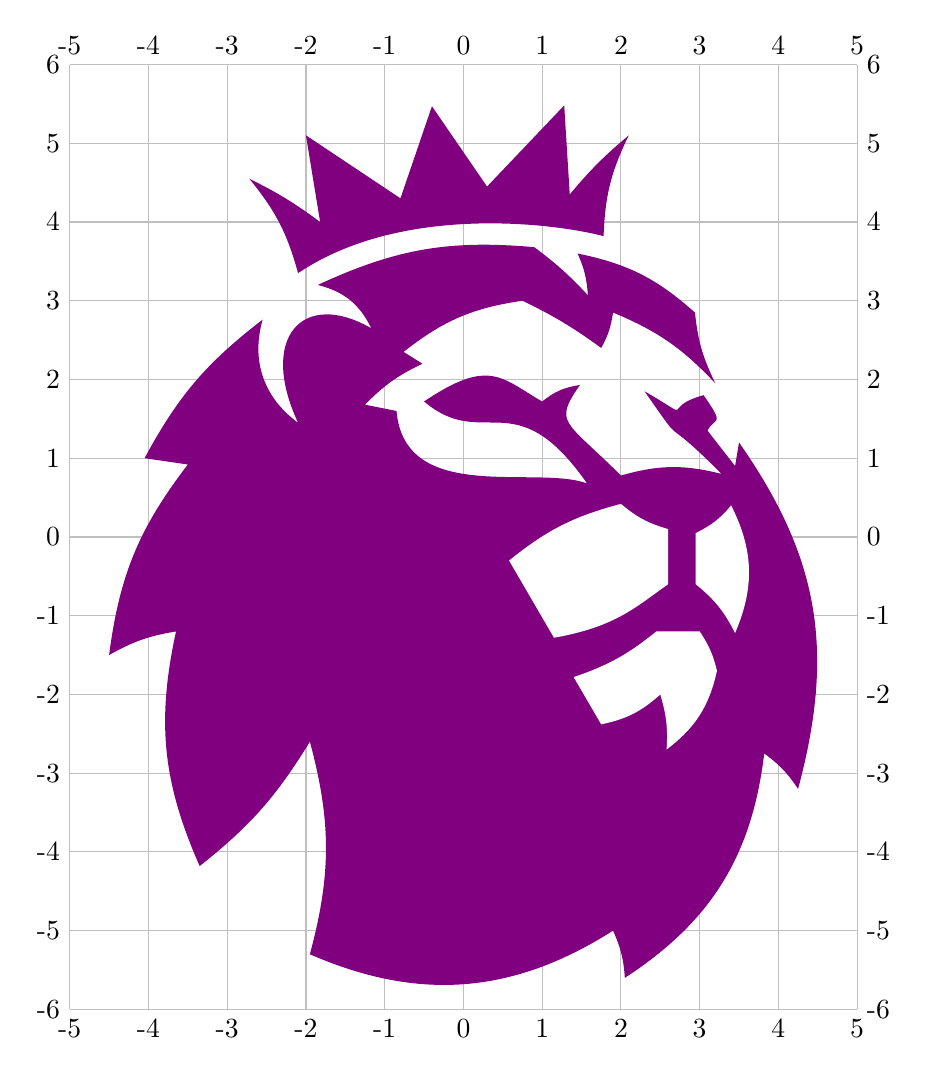
\begin{tikzpicture}
		%\clip (-5,-6) rectangle (5,6);
		%https://www.pngkey.com/detail/u2q8a9y3a9i1r5q8_premier-league-lions-head-vector-logo-premier-league/
		%\node[opacity=.5,scale=.32]{\includegraphics{premier-league}};
		\draw[gray!50] (-5,-6) grid (5,6);
		\fill (0,0) circle(.1);
		\foreach \i in {-5,...,5} \path 
		(\i,-6) node[black,below]{\i}
		(\i,6) node[black,above]{\i};
		\foreach \j in {-6,...,6} \path 
		(-5,\j) node[black,left]{\j}
		(5,\j) node[black,right]{\j};
		
		\fill[violet] (-2.1,3.35) 
		.. controls +(34:1.6) and +(165:.6) .. (1.78,3.82)
		to[bend left=12] (2.1,5.1)
		to[bend right=5] (1.35,4.35)
		--(1.28,5.48)--(.3,4.45)--(-.4,5.47)--
		(-.8,4.3)--(-2,5.1)--(-1.82,4) 
		to[bend right=5] (-2.72,4.55)
		to[bend left=12] cycle
		;
		\fill[violet] (-1.85,3.2) 
		to[bend left=15] (.9,3.68)
		to[bend left=5] (1.58,3.07)
		to[bend right=10] (1.45,3.6)
		to[bend left=15] (2.94,2.85)
		to[bend right=10] (3.2,1.95)
		to[bend right=12] (1.9,2.85)
		to[bend left=10] (1.75,2.4)
		to[bend right=5] (.75,3)
		to[bend right=15] (-.76,2.35)--(-.52,2.2)
		to[bend right=10] (-1.25,1.68)--(-.85,1.6)
		.. controls +(-85:1.2) and +(160:.7) .. (1.57,.68)
		.. controls +(125:1.6) and +(-40:1) .. (-.5,1.72)
		.. controls +(34:1) and +(150:.6) .. (1,1.72)
		to[bend left=15] (1.48,1.93)
		.. controls +(-125:.6) and +(135:1) .. (2,.78)
		to[bend left=15] (3.28,.8)
		.. controls +(135:1.2) and +(-55:1) .. (2.3,1.85)
		.. controls +(-30:.8) and +(-165:.6) .. (3.05,1.8)
		.. controls +(-55:.5) and +(65:.2) .. (3.1,1.35)
		--(3.45,.9)--(3.5,1.2)
		.. controls +(-55:1.8) and +(75:1.8) .. (4.25,-3.2)
		to[bend right=10] (3.82,-2.75)
		to[bend left=25] (2.05,-5.6)
		to[bend right=10] (1.9,-5)
		to[bend left=28] (-1.95,-5.3)
		to[bend right=15] (-1.95,-2.6)
		to[bend left=10] (-3.35,-4.18)
		to[bend left=18] (-3.65,-1.2)
		to[bend right=10] (-4.5,-1.5)
		to[bend left=15] (-3.5,.92)--(-4.05,1)
		to[bend left=12] (-2.55,2.76)
		to[bend right=35] (-2.1,1.45)
		.. controls +(115:1.2) and +(150:1) .. (-1.17,2.65)
		to[bend right=25] cycle
		;
		
		\fill[white] (.58,-.3)
		to[bend left=12] (2,.42)
		to[bend right=12] (2.6,.1)--(2.6,-.6)
		.. controls +(-145:.5) and +(10:.8) .. (1.15,-1.28)
		--cycle;
		\fill[white] (2.95,.05)--(2.95,-.6)
		to[bend left=12] (3.45,-1.22)
		to[bend right=25] (3.4,.4)
		to[bend left=12] cycle
		;
		\fill[white] (1.4,-1.78)--(1.75,-2.38)
		to[bend right=15] (2.5,-2)
		to[bend left=10] (2.58,-2.7)
		to[bend right=20] (3.22,-1.7)
		to[bend right=10] (3,-1.2)--(2.45,-1.2)
		to[bend left=10] cycle
		;
	\end{tikzpicture}
\end{document}